\section{The Koenigs connection}
\label{a:sec:koenigs}

Some time after the search had been abandoned, a dynamical argument emerged that
explains why no elementary closed form should be expected. In short: $A(p)$ is a
value of the Koenigs linearising function of the logistic map, and that function is
known to be non-elementary throughout the parameter range required.

\begin{definition}[Koenigs function]
\label{a:def:koenigs}
Let $f(z) = rz(1-z)$ have a fixed point at $z=0$ with multiplier $r=f'(0)$, and
suppose $|r|\notin\{0,1\}$. Koenigs \cite{Koenigs1884} proved that there is a
unique function $\psi_r$, analytic near the origin, satisfying the Schröder
equation
\begin{equation}
\label{a:eq:schroder}
\psi_r\bigl(f(z)\bigr) = r\,\psi_r(z),
\qquad
\psi_r(0)=0,
\qquad
\psi_r'(0)=1 .
\end{equation}
\end{definition}

\noindent
The Koenigs function is a change of coordinate that straightens the dynamics: in
the $\psi$ coordinate the nonlinear map $f$ becomes multiplication by $r$
(\cref{a:fig:koenigs}). Here $f(z)=rz(1-z)$ is exactly \cref{a:eq:logistic}, with
$z=w_n$ and $f(z)=w_{n+1}$, and the multiplier is $r=2p\in(0,1)$ --- an attracting
fixed point, which is the classical Koenigs setting. Standard accounts are Milnor
\cite{Milnor2006} and Carleson and Gamelin \cite{Carleson1993}.

\begin{figure}[ht]
\centering
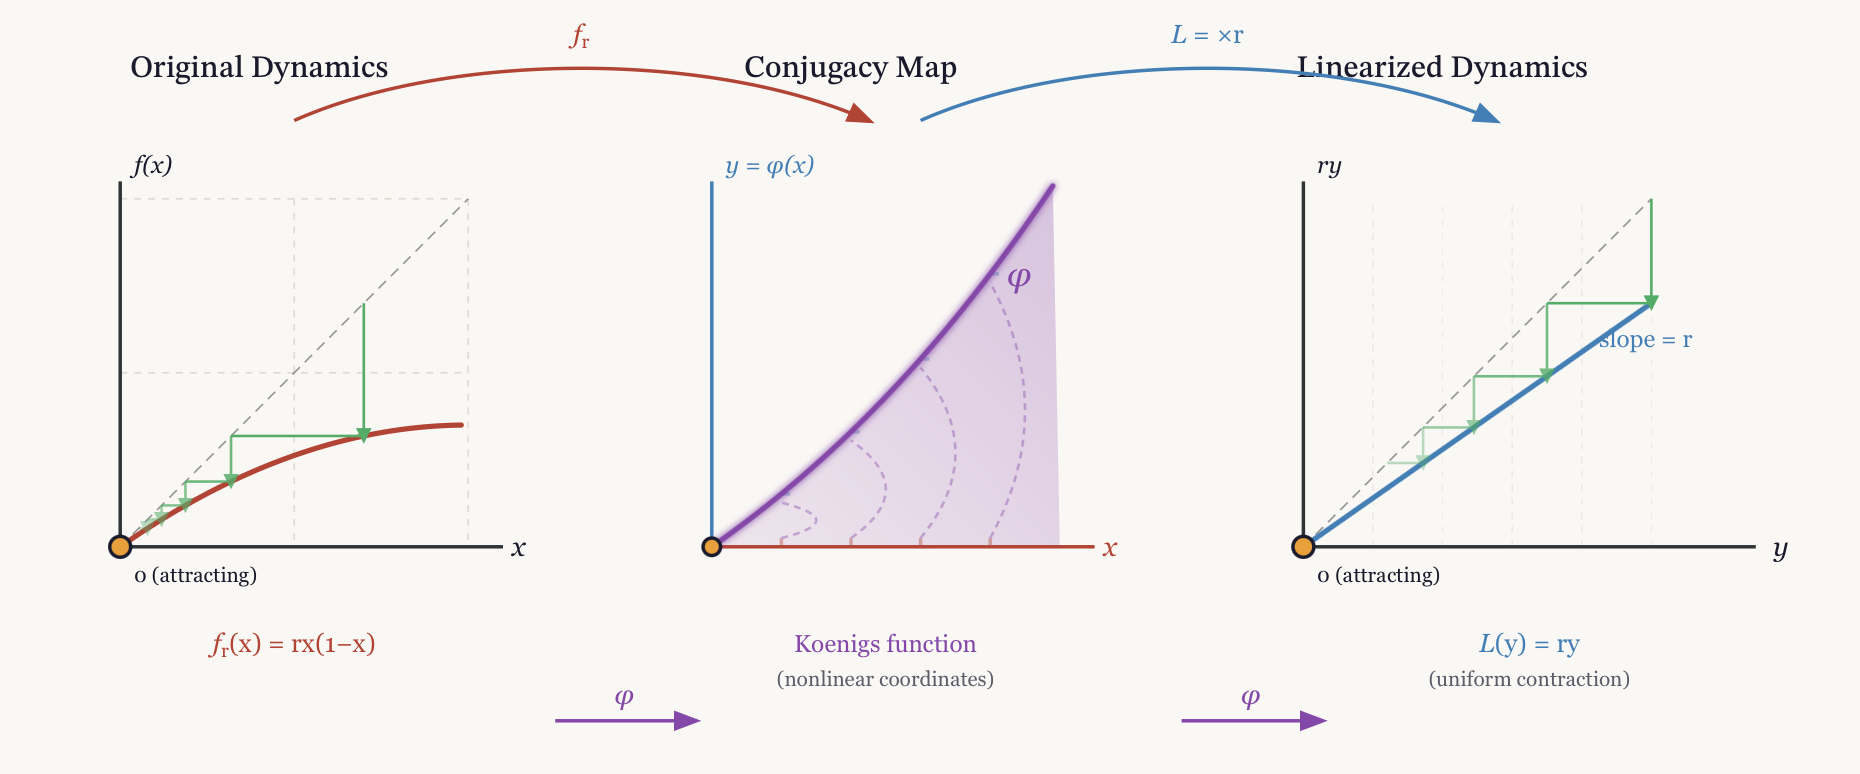
\includegraphics[width=0.72\textwidth]{figures/IMG_ch3/figure2_koenigs_linearization.png}
\caption{Koenigs linearisation of the logistic map near an attracting fixed point.
The nonlinear dynamics $x\mapsto f_r(x)=rx(1-x)$ are conjugated by $\psi_r$ to the
linear map $y\mapsto ry$; the diagram displays the functional relation
$\psi_r(f_r(x)) = r\psi_r(x)$ and the role of $\psi_r$ as the coordinate change
that straightens the dynamics.}
\label{a:fig:koenigs}
\end{figure}

\begin{proposition}
\label{a:prop:AisKoenigs}
For $p\in(0,\tfrac12)$ and $r=2p$,
\begin{equation}
\label{a:eq:AeqKoenigs}
A(p) = 2\,\psi_r\!\lrb{\tfrac12} .
\end{equation}
\end{proposition}

\begin{proof}
Iterating \cref{a:eq:schroder} along the orbit $w_0,w_1,w_2,\dots$ of
\cref{a:eq:logistic} gives $\psi(w_1) = r\psi(w_0)$, hence $\psi(w_0)=\psi(w_1)/r$;
similarly $\psi(w_1)=\psi(w_2)/r$, so $\psi(w_0)=\psi(w_2)/r^2$; and by induction
\begin{equation}
\label{a:eq:induction}
\psi(w_0) = \frac{\psi(w_n)}{r^n}\qquad\text{for every }n .
\end{equation}
Since \cref{a:eq:induction} holds for all $n$ we may pass to the limit,
$\psi(w_0) = \lim_n\psi(w_n)/r^n$. The normalisation $\psi(0)=0$, $\psi'(0)=1$
means $\psi(z)/z\to1$ as $z\to0$, and $w_n = S_n/2\to0$ because $r<1$; replacing
$\psi(w_n)$ by $w_n$ in the limit is therefore legitimate, and
$\psi(w_0) = \lim_n w_n/r^n$. Comparing with \cref{a:eq:Aw} and using
$w_0 = S_0/2 = \tfrac12$ gives $A(p) = 2\psi_r(\tfrac12)$.
\end{proof}

\subsubsection*{Elementary cases and the obstruction}

At the exceptional parameters $r=2$ and $r=4$ --- both \emph{outside} the
branching window $r=2p\in(0,1)$ --- the linearisations are elementary:
\begin{equation}
\label{a:eq:psi2}
\psi_2(x) = -\tfrac12\ln(1-2x),
\qquad
\psi_4(x) = \bigl(\arcsin\sqrt{x}\bigr)^2 .
\end{equation}
Both sit over \emph{repelling} fixed points and are derived in full in
\cref{a:app:integrable}. For $r\in(0,1)$ the fixed point is attracting, and the
precise hypertranscendence theorem is stated in \cref{a:sec:ht}: for every such
$r$, $\psi_r$ is hypertranscendental over $\mathbb{C}(z)$. The softer parameter-plane
observation that $c(r)=(2r-r^2)/4$ avoids $\{0,-2\}$ on $r\in(0,1)$ is true but
logically superfluous once the attracting/repelling dichotomy is in hand
(\cref{a:rem:empty}).

\begin{figure}[ht]
\centering
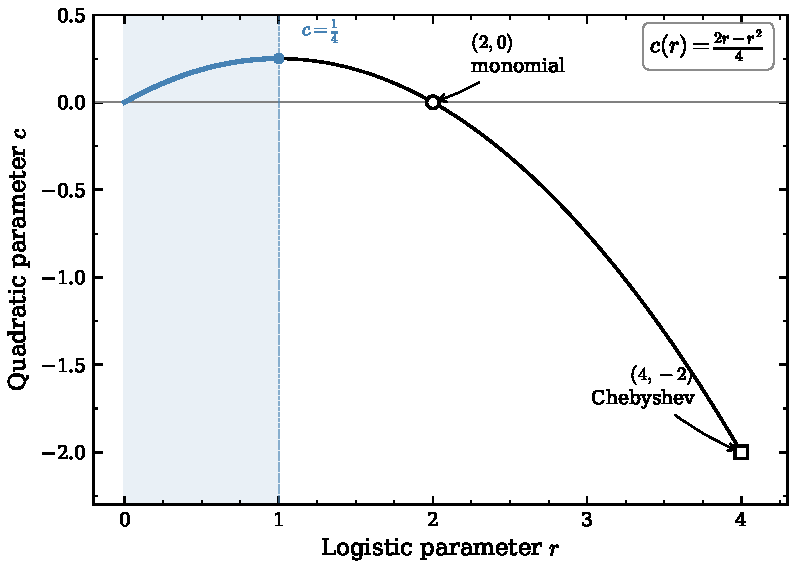
\includegraphics[width=0.66\textwidth]{figures/IMG_ch3/figure1_parameter_conjugacy.pdf}
\caption{The affine parameter correspondence $c(r) = (2r-r^2)/4$ between the
logistic family $f_r(x)=rx(1-x)$ and the quadratic family $P_c(z)=z^2+c$. The
shaded segment is $r\in(0,1)$, the subcritical branching window, which maps to
$c\in(0,\tfrac14)$. The two integrable parameters, $r=2$ ($c=0$, monomial) and
$r=4$ ($c=-2$, Chebyshev), lie outside it.}
\label{a:fig:conjugacy}
\end{figure}

\begin{figure}[ht]
\centering
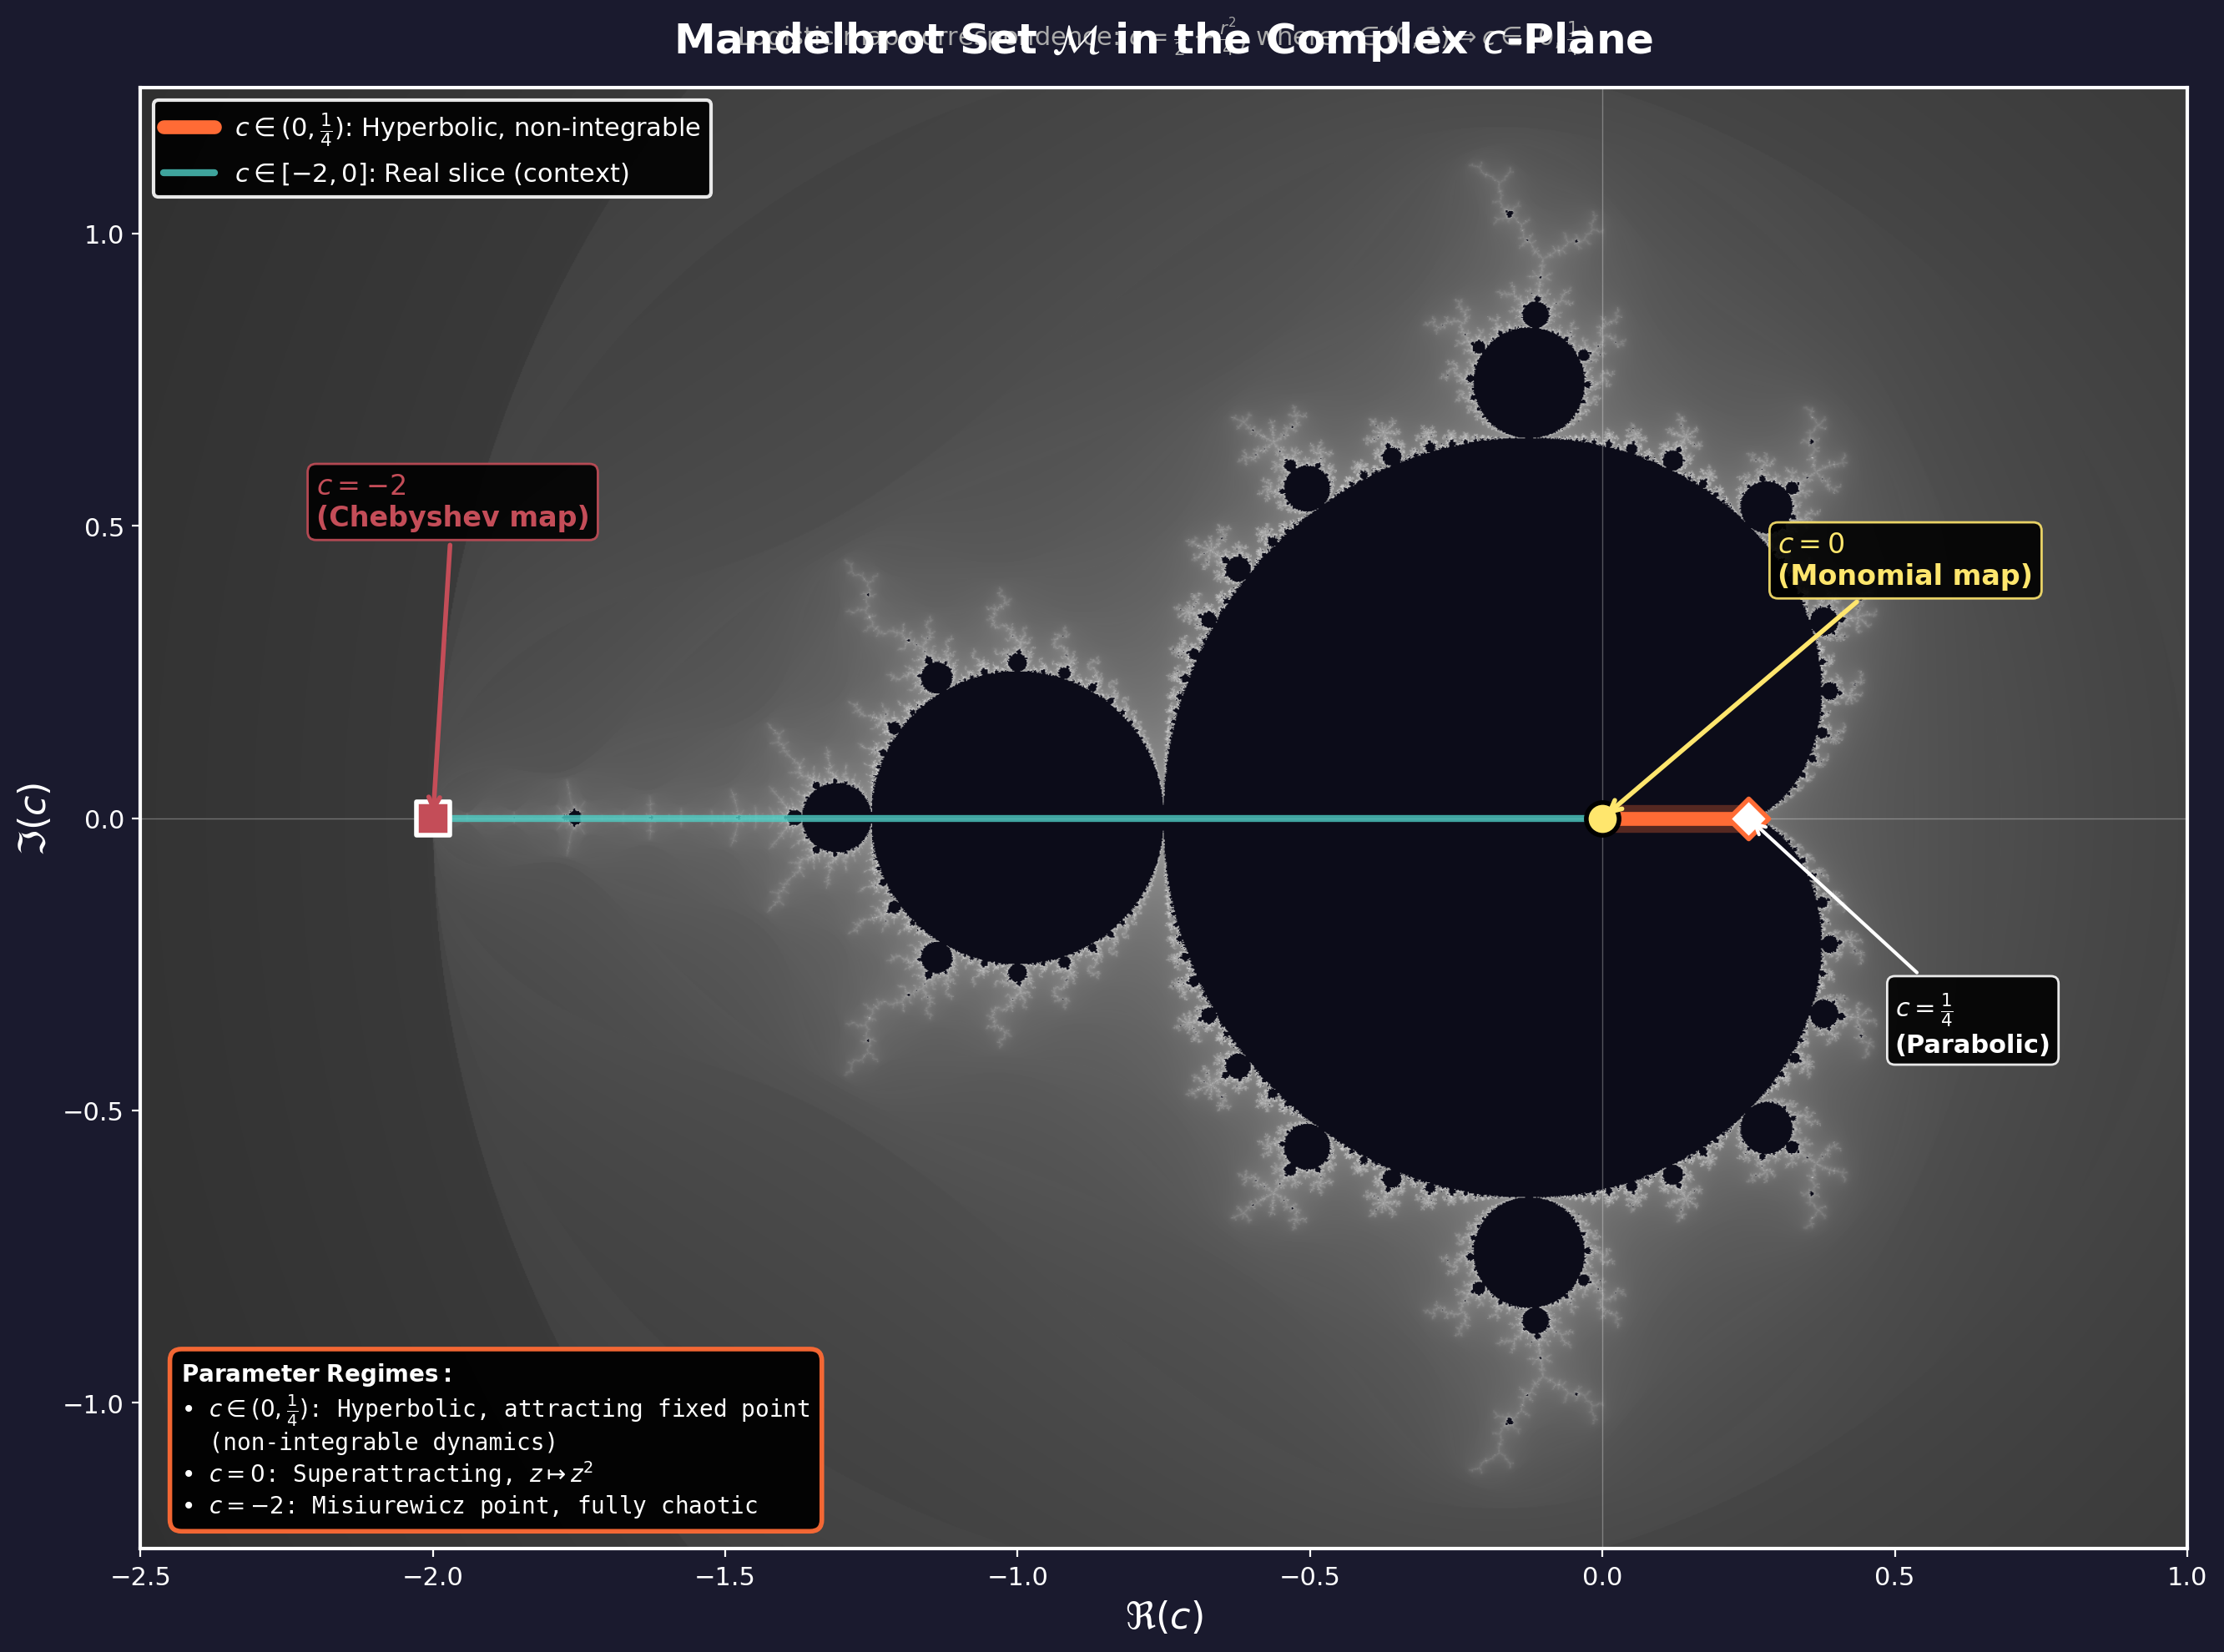
\includegraphics[width=0.92\textwidth]{figures/IMG_ch3/figure4_mandelbrot_context.png}
\caption{The Mandelbrot set in the complex $c$-plane, with the interval
$c\in(0,\tfrac14)$ highlighted. Under the correspondence $c=(2r-r^2)/4$ this is
the image of the subcritical branching window $r=2p\in(0,1)$. Pedagogical context
only: the hypertranscendence proof of \cref{a:sec:ht} does not rely on this picture.}
\label{a:fig:mandelbrot}
\end{figure}
